\documentclass[12pt, a4paper]{article}

\usepackage[margin=1in]{geometry}
\usepackage{graphicx}
\usepackage{hyperref}
\usepackage{booktabs}
\usepackage{parskip}
\usepackage{titlesec}
\usepackage{enumitem}
\usepackage{float}
\usepackage{tikz}
\usetikzlibrary{shapes.geometric, arrows.meta, positioning, fit}

\hypersetup{
    colorlinks=true,
    linkcolor=black,
    urlcolor=blue,
}

\titleformat{\section}{\large\bfseries}{}{0em}{}[\titlerule]
\titleformat{\subsection}{\normalsize\bfseries}{}{0em}{}

\title{
    \textbf{Kafka Lag Analyser} \\[0.4em]
    \large A Plug-and-Play Fault Detection Module for Apache Kafka \\[1em]
    \normalsize CS349 Project Report
}
\author{
    Hari\ (23B0907) \quad
    Tejas\ (23B0932) \quad
    Avinash\ (23B1064) \quad
    Rishi\ (23B1081)
}
\date{May 2026}

\begin{document}

\maketitle
\thispagestyle{empty}

% ────────────────────────────────────────────────────────────────────────────
\section{Overview}

The Kafka Lag Analyser is a plug-and-play monitoring module that can be attached
to any existing Apache Kafka deployment with minimal configuration changes.
Once running, it continuously monitors the cluster and surfaces pre-emptive,
high-signal alerts when it detects one of five known failure patterns.

The design goal is to give a Kafka administrator actionable warnings \textit{before}
a failure cascades into user-visible downtime. Rather than relying on raw metric
thresholds, the system uses trained machine learning models to interpret patterns
across many metrics simultaneously and report a maximum of four concise,
context-rich alerts per incident. It names the affected consumer group or topic
alongside the exact signals that triggered the detection.

Integrating the module into an existing deployment requires exposing the Kafka
broker's JMX metrics via the standard Prometheus JMX Exporter agent. This is
typically a single JVM argument added to the broker's startup configuration.
The scraper and analyser services are then started alongside the cluster using
the provided Docker Compose file.

% ────────────────────────────────────────────────────────────────────────────
\section{Motivation}

A production Kafka cluster emits thousands of metrics: per-topic byte rates,
per-partition log offsets, request latencies broken down by percentile and
request type, consumer group states, replication lag, thread pool utilisation,
and more. In practice, operators set threshold alerts on a handful of these and
watch dashboards for the rest. This approach has two well-known problems. First,
a single fault condition often shows up as correlated anomalies across dozens of
metrics at once---an operator looking at individual graphs has to manually
connect the dots under pressure. Second, threshold-based alerts fire constantly
on healthy clusters with variable load, creating alert fatigue that causes real
problems to be missed. The core idea behind this project is to push the
complexity of interpreting raw metrics into machine learning models, so that the
operator only ever sees the output: a small number of labelled fault events, each
pointing to the specific entity (consumer group, topic, or broker) that is
affected. The human monitors the result of the model, not the metrics themselves.

% ────────────────────────────────────────────────────────────────────────────
\section{Product Specification}

\subsection{Fault Classes}

The system detects five fault classes, each corresponding to a common operational
problem in Kafka deployments:

\begin{enumerate}[leftmargin=*, label=\textbf{Class \arabic*.}]
    \item \textbf{Rebalance Loop} : A consumer group enters a continuous cycle
          of rebalancing without ever stabilising. This typically happens when
          session timeouts are misconfigured, when consumers crash during
          assignment, or when partition topology changes faster than consumers
          can keep up.
    \item \textbf{Broker Saturation} : The broker's CPU or I/O resources are
          exhausted. Produce requests begin to queue, request handler threads
          become idle waiting for disk, and throttle times spike.
    \item \textbf{Network Degradation} : Elevated latency between the broker
          and clients, or between brokers in a replicated cluster. Under-replicated
          partitions appear and inter-broker replication lag grows.
    \item \textbf{Partition Skew} : Write traffic is concentrated on a subset
          of partitions of a topic while others are idle. This causes uneven
          storage growth and hot-spot latency for the partitions absorbing all
          traffic.
    \item \textbf{Slow Consumer} : A consumer group is processing messages
          slower than producers are writing them. Lag grows monotonically rather
          than fluctuating around a steady state.
\end{enumerate}

These classes were chosen so that they are operationally meaningful and also are disjoint in their causes. 
This makes it easier for the models to learn to distinguish between different fault types.

\subsection{User Interaction Model}

Figure~\ref{fig:user-flow} shows how an operator interacts with the system.

\begin{figure}[H]
\centering
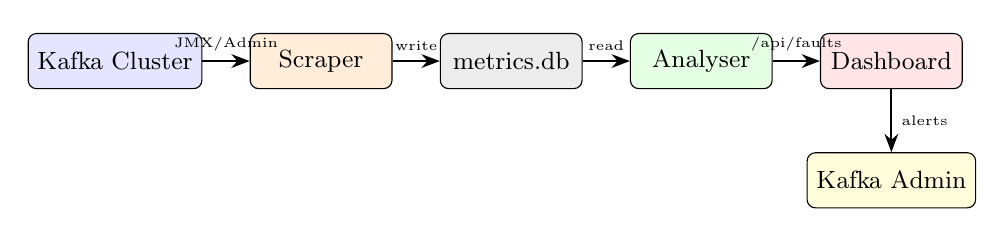
\begin{tikzpicture}[
    node distance=0.8cm and 0.6cm,
    box/.style={rectangle, draw, rounded corners=3pt, minimum width=1.8cm,
                minimum height=0.7cm, text centered, font=\small},
    arr/.style={-Stealth, thick},
]
    \node[box, fill=blue!10]  (kafka)    {Kafka Cluster};
    \node[box, fill=orange!15, right=of kafka] (scraper)  {Scraper};
    \node[box, fill=gray!15,   right=of scraper] (db)      {metrics.db};
    \node[box, fill=green!10,  right=of db]      (analyser){Analyser};
    \node[box, fill=red!10,    right=of analyser](ui)      {Dashboard};
    \node[box, fill=yellow!15, below=of ui]      (admin)   {Kafka Admin};

    \draw[arr] (kafka)    -- node[above, font=\tiny]{JMX/Admin} (scraper);
    \draw[arr] (scraper)  -- node[above, font=\tiny]{write} (db);
    \draw[arr] (db)       -- node[above, font=\tiny]{read} (analyser);
    \draw[arr] (analyser) -- node[above, font=\tiny]{/api/faults} (ui);
    \draw[arr] (ui)       -- node[right, font=\tiny]{alerts} (admin);
\end{tikzpicture}
\caption{End-to-end data flow from Kafka cluster to the operator dashboard.}
\label{fig:user-flow}
\end{figure}

The operator opens \texttt{http://localhost:8000} in a browser. The dashboard
auto-refreshes every three seconds. If all models report healthy, a green banner
is shown. When a model fires, a red card appears naming the fault class, the
affected entity (e.g.\ \texttt{consumer\_group=my-app}), and a collapsible
panel showing the exact metric values that triggered the detection.

% ────────────────────────────────────────────────────────────────────────────
\section{System Architecture}

The system is composed of four services, all orchestrated with Docker Compose:

\begin{enumerate}[leftmargin=*, label=\textbf{\arabic*.}]
    \item \textbf{Kafka Broker} : KRaft cluster with the Prometheus
          JMX Exporter Java agent attached. The exporter filters and renames
          JMX MBeans into Prometheus-format metrics and exposes them on port
          \texttt{9101}.
    \item \textbf{Scraper} : A Python service that polls the JMX exporter
          endpoint and the Kafka Admin API every 10 seconds. Each poll collects
          broker-level JMX metrics and per-partition consumer lag for all active
          consumer groups, then writes both into an SQLite database
          (\texttt{data/metrics.db}) shared via a host volume mount.
    \item \textbf{Analyser} : A FastAPI service that wakes up every 10 seconds,
          loads the last 100 seconds of scrape data from the shared database,
          runs feature extraction, and feeds the resulting feature vectors into
          each trained XGBoost model. Any model predicting a fault (output = 1)
          produces a fault event that is stored in memory and served from
          \texttt{/api/faults}.
    \item \textbf{Dashboard} : A static HTML/JS page served by the Analyser.
          It polls \texttt{/api/faults} every three seconds and renders the
          current fault state and a rolling history of the last 200 events.
\end{enumerate}

\subsection{Training Pipeline}

Training is offline and separate from the runtime system.
Figure~\ref{fig:train-pipeline} shows the pipeline.

\begin{figure}[H]
\centering
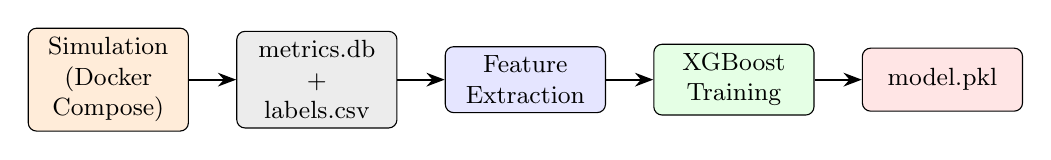
\begin{tikzpicture}[
    node distance=0.7cm and 0.6cm,
    box/.style={rectangle, draw, rounded corners=3pt, minimum width=2.0cm,
                minimum height=0.8cm, text width=1.8cm, align=center, font=\small},
    arr/.style={-Stealth, thick},
]
    \node[box, fill=orange!15] (sim)    {Simulation\\(Docker Compose)};
    \node[box, fill=gray!15, right=of sim]  (db)     {metrics.db +\\labels.csv};
    \node[box, fill=blue!10, right=of db]   (feat)   {Feature\\Extraction};
    \node[box, fill=green!10, right=of feat](train)  {XGBoost\\Training};
    \node[box, fill=red!10, right=of train] (pkl)    {model.pkl};

    \draw[arr] (sim)   -- (db);
    \draw[arr] (db)    -- (feat);
    \draw[arr] (feat)  -- (train);
    \draw[arr] (train) -- (pkl);
\end{tikzpicture}
\caption{Offline training pipeline. One model is trained per fault class.}
\label{fig:train-pipeline}
\end{figure}

For each fault class, a simulation script spins up a local Kafka environment
using Docker Compose (including a producer and a consumer) and deliberately
induces the target fault condition. The scraper runs throughout, writing metrics
into a \texttt{metrics.db}. Once the simulation ends, a \texttt{labels.csv} is
generated that marks each scrape session as either \texttt{healthy} or the
relevant fault class. The simulation methodology per class is as follows:

\begin{itemize}
    \item \textbf{Rebalance Loop} - The simulation sends repeated consumer
          reconnection commands and induces session timeouts at 5-second
          intervals, then incrementally adds topic partitions to force
          continuous rebalancing.
    \item \textbf{Broker Saturation} - The broker container's CPU is throttled
          to 5\% of a core using Docker resource limits, while the producer
          sends 5\,MB random-byte payloads to simultaneously stress disk I/O.
    \item \textbf{Network Degradation} - Linux traffic control (\texttt{tc
          netem}) injects 400\,ms of latency on the inter-broker network
          interface and 200\,ms on client-facing interfaces, degrading both
          replication and client round-trip times. Note: the training data for 
          this class was flawed due to missing JMX exporter rules, so the model 
          trained on it is not valid.
    \item \textbf{Partition Skew} - The producer is configured to put all
          writes to a subset of partitions.
    \item \textbf{Slow Consumer} - The consumer's processing rate is
          artificially throttled to 20\% of the producer's write rate.
\end{itemize}

Features are extracted from the raw time-series data by computing rolling
statistics (slopes, standard deviations, coefficient of variation) over a
window. This transforms point-in-time snapshots into trend-aware
signals. Each model is then trained using XGBoost with five-fold stratified
cross-validation and class-balanced sample weights. The trained models are
serialised as \texttt{.pkl} files and mounted into the analyser container at
runtime.

\subsection{Inference Pipeline}

Figure~\ref{fig:infer-pipeline} shows the runtime inference pipeline.

\begin{figure}[H]
\centering
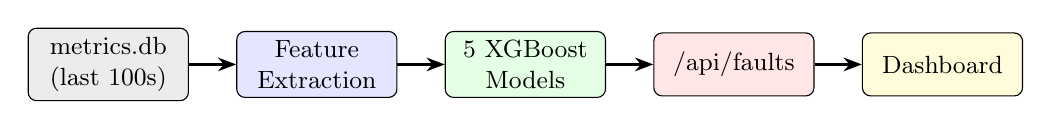
\begin{tikzpicture}[
    node distance=0.7cm and 0.6cm,
    box/.style={rectangle, draw, rounded corners=3pt, minimum width=2.0cm,
                minimum height=0.8cm, text width=1.8cm, align=center, font=\small},
    arr/.style={-Stealth, thick},
]
    \node[box, fill=gray!15]   (db)    {metrics.db\\(last 100s)};
    \node[box, fill=blue!10, right=of db]   (feat)  {Feature\\Extraction};
    \node[box, fill=green!10, right=of feat](models){5 XGBoost\\Models};
    \node[box, fill=red!10, right=of models](api)   {/api/faults};
    \node[box, fill=yellow!15, right=of api](dash)  {Dashboard};

    \draw[arr] (db)    -- (feat);
    \draw[arr] (feat)  -- (models);
    \draw[arr] (models)-- (api);
    \draw[arr] (api)   -- (dash);
\end{tikzpicture}
\caption{Runtime inference pipeline, repeated every 10 seconds.}
\label{fig:infer-pipeline}
\end{figure}

\subsection{Model Performance}

Table~\ref{tab:f1} shows the mean cross-validation F1 score (fault class = 1)
for each trained model.

\begin{table}[H]
\centering
\begin{tabular}{lcc}
\toprule
\textbf{Fault Class}   & \textbf{CV F1 (fault)} & \textbf{Note} \\
\midrule
Slow Consumer          & 0.98 & \\
Partition Skew         & 0.99 & \\
Rebalance Loop         & 0.87 & \\
Broker Saturation      & 0.78 & \\
Network Degradation    & 0.11 & Training data issue (see below) \\
\bottomrule
\end{tabular}
\caption{5-fold stratified cross-validation F1 scores per fault class.}
\label{tab:f1}
\end{table}

Four of the five models perform well. The network degradation model scores
poorly because the simulation data for that class contained near-zero values for
all latency and throughput metrics --- the JMX exporter rules for several key
metrics (\texttt{RemoteTimeMs}, \texttt{ResponseSendTimeMs}, throughput counters)
were missing from the exporter configuration at the time of data collection,
meaning the broker never published those metrics and the scraper stored zeros.
The model has nothing to split on. Retraining after fixing the exporter
configuration is the immediate remediation.

% ────────────────────────────────────────────────────────────────────────────
\section{Testing}

The system was tested on a demo cluster whose workload can be varied using the
same configurable knobs as the training simulations. To evaluate a given fault
class, the corresponding fault knob is activated and the dashboard is observed
to confirm that the correct fault card appears within one to two analysis cycles
(10--20 seconds). Returning the knob to the healthy state should cause the
alert to clear on the next cycle. This procedure was carried out for each of the
four well-trained fault classes.

The demo cluster was also run in a sustained healthy state for an extended
period to check for spurious alerts. No false positives were observed during
this period for the slow consumer, partition skew, and rebalance loop models.
The broker saturation model occasionally fired false positives under normal
load spikes, which is consistent with its lower F1 score and the relatively
coarse features available for that class.

% ────────────────────────────────────────────────────────────────────────────
\section{Use of AI}

GitHub Copilot was used extensively throughout this project. The primary use was
code generation: Copilot was prompted with descriptions of what each module
needed to do (e.g.\ ``write a FastAPI endpoint that loads recent scrape data
from SQLite and runs XGBoost inference''), and the generated code was reviewed,
corrected, and \textbf{integrated} by the us. Architecture decisions were made by 
the us and then implemented with Copilot assistance.

Copilot was also used for debugging.

% ────────────────────────────────────────────────────────────────────────────
\section{Future Work}

\begin{itemize}
    \item \textbf{Network degradation retraining.} The most urgent next step is
          fixing the JMX exporter configuration for the missing metric rules and
          re-running the class 3 simulation to produce a valid training dataset.
    \item \textbf{Online model updating.} Models are trained offline on
          simulations. A mechanism to periodically retrain on data collected from
          the live cluster would allow the models to adapt to deployment-specific
          traffic patterns.

    \item \textbf{Root-cause ranking.} When multiple models fire simultaneously,
          there is currently no ranking of which fault is most likely primary.
          Adding a confidence score to each fault event (e.g.\ using XGBoost's
          \texttt{predict\_proba}) would allow the dashboard to surface the
          highest-confidence alert first.
\end{itemize}

\end{document}
